%! Author = Charles Yang

% Preamble
\documentclass[11pt]{article}

% Packages
\usepackage{amsmath}
\usepackage{amsfonts}
\usepackage{hyperref}
\usepackage{enumitem}
\usepackage{graphicx}

% Settings
\setlist[enumerate]{font=\bfseries}

% Title Info
\title{STAT 347 HW3}
\author{Charles Yang}

\addtolength{\oddsidemargin}{-.875in}
\addtolength{\evensidemargin}{-.875in}
\addtolength{\textwidth}{1.75in}
\addtolength{\topmargin}{-.875in}
\addtolength{\textheight}{1.75in}

% Document
\begin{document}
    \maketitle

    \begin{enumerate}
        \item[3.38]
        \begin{enumerate}
            \item[a] $P(Y = y) = C(4,y)(1/3)^{y}(2/3)^{4-y}$
            \item[b] $P(Y \geq 3) = P(3) + P(4) = C(4,3)(1/3)^{3}(2/3)^{1} + C(4,4)(1/3)^{4}(2/3)^{0} = 1/9$
            \item[c] $4*1/3 = 4/3$
            \item[d] $4*(1/3)*(2/3) = 8/9$
        \end{enumerate}

        \item[3.40]
        \begin{enumerate}
            Looking at appendix 3 table 1 for $p = 0.8$ and $n = 20$
            \item[a] $C(20,14)(0.8)^{14}(0.2)^6$
            \item[b] $P(Y \leq 9)$. $P(Y \geq 10) = 1 - P(Y \leq 9) = 1- 0.001 = 0.999$. Or $1- \sum_{y=0}^{9} C(20, y)(0.8)^y(0.2)^{20-y}$
            \item[c] $P(Y \leq 18) - P(Y \leq 13) = 0.931 - 0.087 = 0.844$. Or $\sum_{y=14}^{18} C(20, y)(0.8)^y(0.2)^{20-y}$
            \item[d] $P(Y \leq 16) = 0.589$. Or $1 - \sum_{y=17}^{20} C(20, y)(0.8)^y(0.2)^{20-y}$
        \end{enumerate}

        \item[3.41] Looking at appendix 3 table 1 for $n = 15$, $p = 0.2$ \\
        $P(Y \geq 10) = 1 - P(Y \leq 9) = \sim0$. Or $\sum_{y = 10}^{15} C(15, y)(0.2)^y(0.8)^{15-y}$

        \item[3.44]
        \begin{enumerate}
            \item[a] $0.8^5 = 0.3277$
            \item[b] $C(5, 4)(0.6)^4(0.4)$
            \item[c] $C(5, 1)(0.6)(0.4)^4 + C(5, 2)(0.6)^2(0.4)^3$
        \end{enumerate}

        \item[3.46] Using appendix 3 table 1 as suggested: \\
        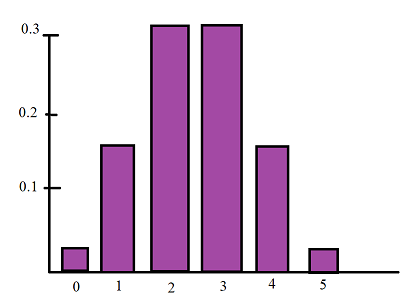
\includegraphics{pain.png}

        \newpage

        \item[3.60]
        \begin{enumerate}
            \item[a] $C(20,14)(0.8)^{14}(0.2)^6$
            \item[b] $\sum_{y = 10}^{20} C(20,y)(0.8)^{y}(0.2)^{20 - y}$
            \item[c] $1 - \sum_{y = 17}^{20} C(20,y)(0.8)^{y}(0.2)^{20 - y}$
            \item[d] $\sigma^2 = 20(1/5)(4/5) = 80/25 = 16/5$, $E(Y) = 20(0.8) = 16$
        \end{enumerate}

        \item[3.66]
        \begin{enumerate}
            \item[a]
            \begin{align*}
                \sum_{y} p(y) &= \sum_{y=1}^{\infty} q^{y - 1}p \\
                &= p \sum_{y=1}^{\infty} q^{y - 1} \\
                &= p \sum_{y=0}^{\infty} q^{y} \\
                &= p \frac{1}{1-q} \\
                &= p \frac{1}{1-(1 - p)} \\
                &= p \frac{1}{p} \\
                &= 1
            \end{align*}
            \item[b] 0, because p(y) decreases as y increases
        \end{enumerate}

        \item[3.70]
        \begin{enumerate}
            \item[a] $(0.2)(0.8)^2$
            \item[b] $0.8^{10}$
        \end{enumerate}

        \item[3.73]
        \begin{enumerate}
            \item[a] $(0.9)(0.1)^2$
            \item[b] $0.9\sum_{y=3}^{\infty} (0.1)^{y - 1} = 0.9 \frac{0.01}{1 - 0.1} = 0.9 \frac{0.01}{0.9} = 0.01$
        \end{enumerate}

        \item[3.81] $1/(0.5) = 2$

        \item[3.90] $C(10 - 1, 3 - 1)(0.6)^7(0.4)^3$

        \item[3.97]
        \begin{enumerate}
            \item[a] $(0.8)^2(0.2)$
            \item[b] $C(7 - 1, 3 - 1)(0.8)^{4}(0.2)^3$
            \item[c] We assume that every drill probability is independent, the same, and follows a negative binomial probability.
            \item[d] $E(Y) = 3/0.2 = 15$, $V(Y) = 3(0.8)/(0.2)^2 = 60$
        \end{enumerate}

    \end{enumerate}
\end{document}